\documentclass[a4paper,12pt]{report}
\usepackage[utf8]{inputenc}
\usepackage{amsmath} % For mathematical symbols and environments
\usepackage{graphicx} % For including graphics
\usepackage{geometry} % For adjusting page margins
\usepackage{listings}
\usepackage{xcolor}
\usepackage{enumitem} % For customizing lists
\usepackage{float}


% Define the style for C code
\lstset{
    language=C,
    basicstyle=\ttfamily\small,  % Set the basic font style
    keywordstyle=\color{blue},   % Color of keywords
    commentstyle=\color{green},  % Color of comments
    stringstyle=\color{red},     % Color of strings
    numberstyle=\tiny\color{gray}, % Line numbers
    frame=single,                % Frame around the code
    breaklines=true,             % Break long lines
}

\renewcommand{\thesection}{\arabic{section}}
% Set custom margins
\geometry{
  top=1in,    % Top margin
  bottom=1in, % Bottom margin
  left=1in, % Left margin
  right=1in % Right margin
}
% Define custom title format with subtitle and roll number
\title{
  \vspace{-2em} % Adjust the space above the title
  \textbf{CS-700 Algorithms and Complexity} \\ % Main title
  \large \textbf{Assignment-1} \\ % Subtitle
  \vspace{1em} % Space between subtitle and author
  \textbf{ANAND M K} \\ % Author
  Roll Number: 242CS008 % Roll number
}

\date{} % Remove the date

\begin{document}

\maketitle

\section{Introduction}
In this assignment, I have analyzed and compared different sorting algorithms based on their execution time. The performance of these algorithms was compared with varying input sizes, and an in-depth analysis has been conducted.

The following sorting algorithms were considered for comparison:
\begin{itemize}
  \item Bubble Sort
  \item Insertion Sort
  \item Merge Sort
  \item Quick Sort
  \item Heap Sort
  \item Radix Sort
\end{itemize}

\section{Data Generation and Experimental Setup}
\subsection{Input Data}
Three different versions of input data were considered for each algorithm:
\begin{enumerate}
  \item Elements sorted in increasing order.
  \item Elements sorted in decreasing order.
  \item Randomly generated elements.
\end{enumerate}

The program can read the input from a file and execute the code. The format of the input files is as follows:
\begin{verbatim}
[n] //number of positive integers to sort
[element 1]
[element 2]
...
...
[element n]
\end{verbatim}

Where \( n \) varies from 10,000 to 100,000, with intervals of 10,000. For each version of input data, there are 10 input files, each corresponding to a different input data size ranging from 10,000 to 100,000. This varied dataset allows for a more comprehensive analysis.

\newpage
\subsection{Machine Specifications}
\begin{itemize}
  \item CPU: 11th Gen Intel® Core™ i5-11500 @ 2.70GHz × 12
  \item RAM: 16 GB
  \item Operating System: Ubuntu 22.04.4 LTS
  \item Compiler: gcc 11.4.0
\end{itemize}

\subsection{Timing Mechanism}
Execution time was calculated in milliseconds using the gettimeofday() function in C, which provides higher precision than the clock() function. The <sys/time.h> header file is required for gettimeofday(). The following code was used to calculate the execution time.
\begin{lstlisting}
    struct timeval start, end;
    gettimeofday(&start, NULL);
    Sorting Algorithm();
    gettimeofday(&end, NULL);
    double executiontime = (end.tv_sec - start.tv_sec) + ((end.tv_usec - start.tv_usec) / 1000000.0); // Execution time in seconds
    executiontime = executiontime * 1000; // Execution time in milli seconds
\end{lstlisting}

\subsection{Experiment Repetitions}
Each experiment was repeated more than 10 times to verify that the measurements were valid and did not produce incorrect values.

\subsection{Time Capture}
Each sorting algorithm was executed with different input sizes, and the time was captured for each case. The time was calculated as the average of multiple repetitions of the experiments. 

\subsection{Input Generation and Selection}
I have generated the input files as follows:

\begin{itemize}[label=--]
    \item \textbf{For the increasing order file:} Numbers were generated from 100,000 to 100,000 plus the size of the input file.\\
    \textit{Example:} For an increasing order file with 20,000 numbers, the values will range from 100,000 to 120,000.
    
    \item \textbf{For the decreasing order file:} Numbers were generated from 200,000 to 200,000 minus the size of the input file.\\
    \textit{Example:} For a decreasing order file with 20,000 numbers, the values will range from 200,000 to 180,000.
    
    \item \textbf{For the file with random values:} Numbers were generated using the \texttt{rand()} function in C, with values between 100,000 and 200,000.
\end{itemize}

\subsection{Input Consistency: Were the same inputs used for all sorting algorithms?}
Yes, the same set of inputs was used for all sorting algorithms.

\section{Analysis of QuickSort}
Three versions of QuickSort have been considered for analysis:
\begin{itemize}
    \item \textbf{Version 1:} The first element in the array.
    \item \textbf{Version 2:} A random element in the array.
    \item \textbf{Version 3:} The median of the first, middle, and last elements in the array.
\end{itemize}

\subsection{Version 1 : QuickSort with the Pivot as the First Element} 

\begin{itemize}
    \item \textbf{Sorted List in Increasing Order:} Since the pivot is selected as the first element, each partitioning step is highly unbalanced. Therefore, the time complexity results in \(O(n^2)\).
    
    \item \textbf{Sorted List in Decreasing Order:} Similar to the increasing order list, the pivot choice leads to highly unbalanced partitions. Thus, the time complexity also results in \(O(n^2)\).
    
    \item \textbf{Random Order List:} In this case, the list is not sorted, so the pivot does not consistently produce unbalanced partitions. As a result, the algorithm performs better, and the time complexity is approximately \(O(n \log n)\).
\end{itemize}
\begin{figure}[H]
    \centering
    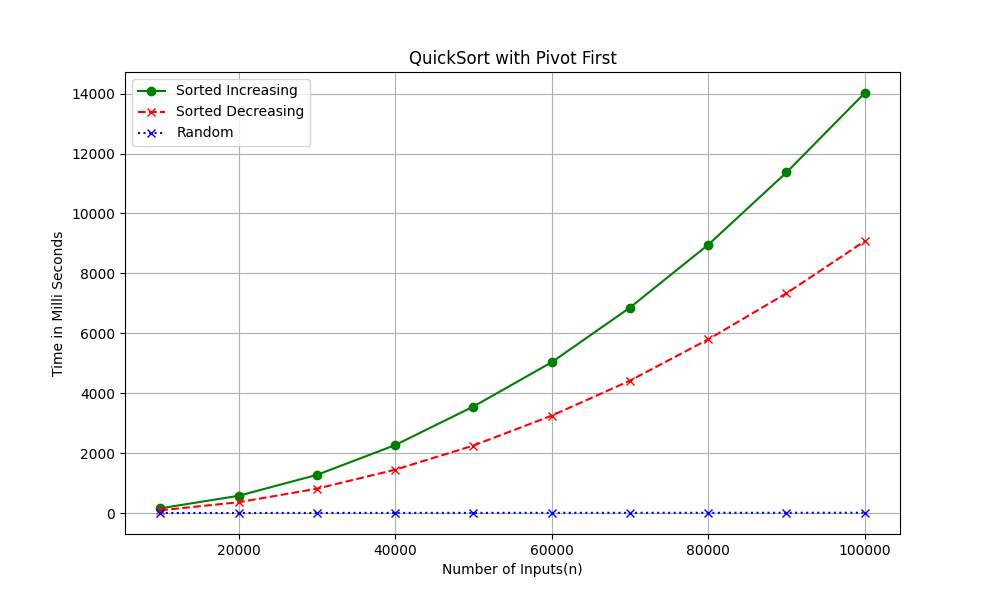
\includegraphics[width=1\textwidth]{./QuickSortPivotFirst.png}
    \caption{Performance of QuickSort with Pivot as the First Element}
    \label{fig:quicksort_performance}
\end{figure}

\subsection{Version 2 : QuickSort with the Pivot as the Random Element} 

\begin{itemize}
    \item \textbf{Sorted List in Increasing Order:} Since the pivot is chosen randomly, each partitioning step is less likely to be highly unbalanced. This results time complexity of \(O(n \log n)\). 
    
    \item \textbf{Sorted List in Decreasing Order:} Similar to the sorted increasing order list, the random pivot selection helps avoid consistently poor partitioning. Therefore, the time complexity is \(O(n \log n)\). 

    \item \textbf{Random Order List:} The random pivot selection generally provides balanced partitions and ensures good performance. The  time complexity is \(O(n \log n)\)
\end{itemize}
\begin{figure}[H]
    \centering
    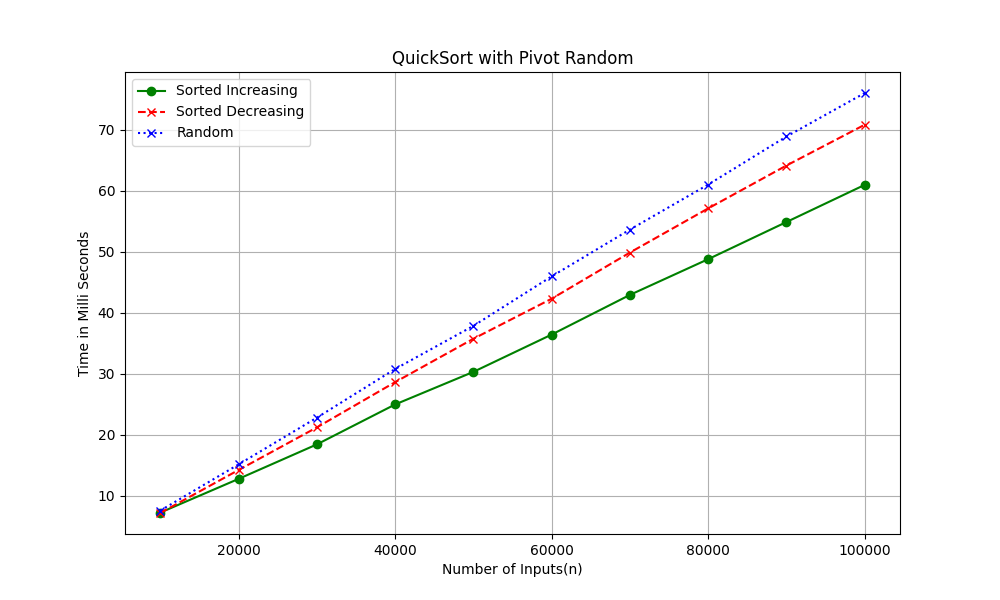
\includegraphics[width=1\textwidth]{./QuickSortPivotRandom.png}
    \caption{Performance of QuickSort with Random Pivot Choice}
    \label{fig:quicksort_random_pivot}
\end{figure}

\subsection{Version 3 : QuickSort with the Pivot as the Median of the First, Middle, and Last Elements} 
\begin{itemize}
    \item \textbf{Sorted List in Increasing Order:} The median of the first, middle, and last elements as the pivot generally results in more balanced partitions, as it chooses a pivot more likely to be near the middle value. This results in an average time complexity of \(O(n \log n)\). 

    \item \textbf{Sorted List in Decreasing Order:}  Similar to the increasing order list, the median as the pivot choice improves partitioning, and the time complexity results in \(O(n \log n)\).

    \item \textbf{Random Order List:} The median pivot selection generally provides balanced partitions and ensures good performance. The time complexity is \(O(n \log n)\).
\end{itemize}

\begin{figure}[H]
    \centering
    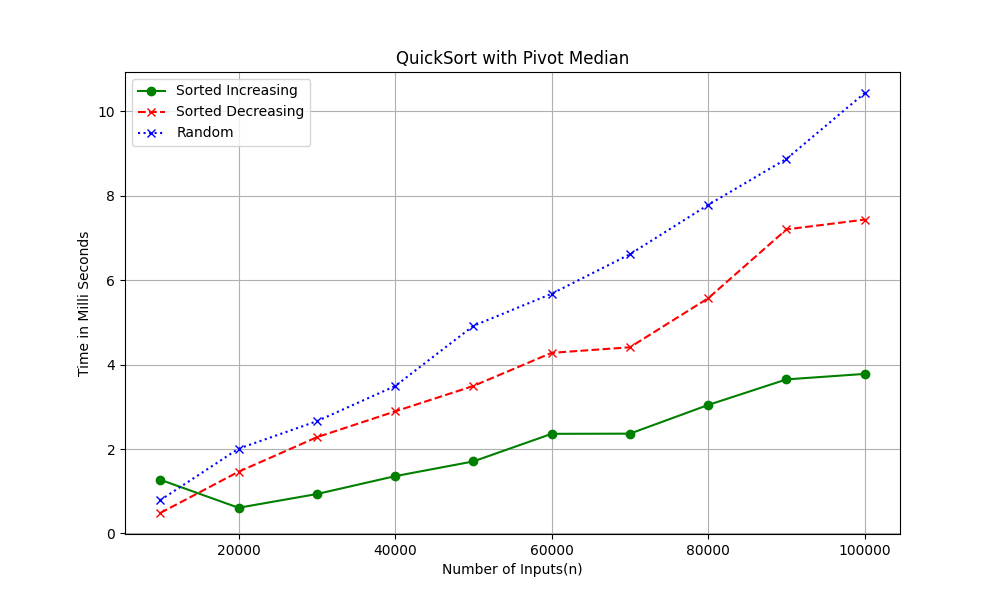
\includegraphics[width=1\textwidth]{./QuickSortPivotMedian.png}
    \caption{Performance of QuickSort with Pivot as the Median of the First, Middle, and Last Elements}
    \label{fig:quicksort_median_pivot}
\end{figure}

\subsection{Best Case Performance of Three Versions of Quick Sort}
As per the above analysis, the best case occurs when the partitions are balanced, and there are fewer unbalanced partitions. This leads to a best-case time complexity of \(O(n \log n)\) in all three versions.
\begin{itemize}
    \item \textbf{Version 1:} As per the above experiments and observations, the random array gives the best case.

    \item \textbf{Version 2:} Even though all types of inputs result in \(O(n \log n)\), considering the experiments conducted and the graph, the sorted array in increasing order gives the best times.

    \item \textbf{Version 3:} Even though all types of inputs result in \(O(n \log n)\), considering the experiments conducted and the graph, the sorted array in increasing order gives the best times.
\end{itemize}

\begin{figure}[H]
    \centering
    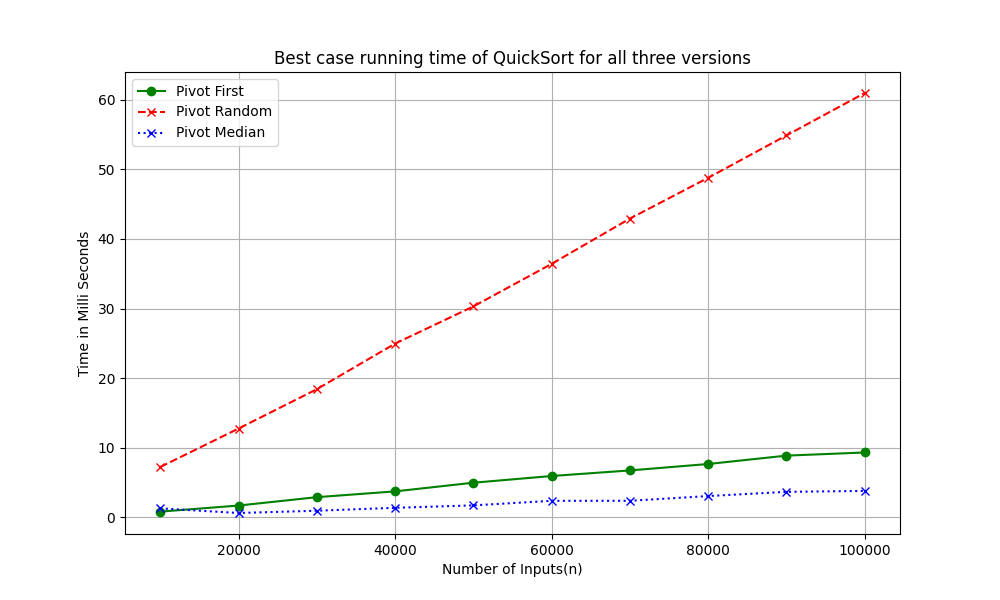
\includegraphics[width=1\textwidth]{./Best_case_QuickSort.png}
    \caption{Best case running time of QuickSort for all three versions}
    \label{fig:quicksort_median_pivot}
\end{figure}


\end{document}
